%!TEX TS-program = xelatex
\documentclass[11pt]{article}

\usepackage[english]{babel}

\usepackage{amsmath,amssymb,amsfonts}
\usepackage[utf8]{inputenc}
\usepackage[T1]{fontenc}
\usepackage{stix2}
\usepackage[scaled]{helvet}
\usepackage[scaled]{inconsolata}

\usepackage{lastpage}

\usepackage{setspace}

\usepackage{ccicons}

\usepackage[hang,flushmargin]{footmisc}

\usepackage{geometry}

\setlength{\parindent}{0pt}
\setlength{\parskip}{6pt plus 2pt minus 1pt}

\usepackage{fancyhdr}
\renewcommand{\headrulewidth}{0pt}\providecommand{\tightlist}{%
  \setlength{\itemsep}{0pt}\setlength{\parskip}{0pt}}

\makeatletter
\newcounter{tableno}
\newenvironment{tablenos:no-prefix-table-caption}{
  \caption@ifcompatibility{}{
    \let\oldthetable\thetable
    \let\oldtheHtable\theHtable
    \renewcommand{\thetable}{tableno:\thetableno}
    \renewcommand{\theHtable}{tableno:\thetableno}
    \stepcounter{tableno}
    \captionsetup{labelformat=empty}
  }
}{
  \caption@ifcompatibility{}{
    \captionsetup{labelformat=default}
    \let\thetable\oldthetable
    \let\theHtable\oldtheHtable
    \addtocounter{table}{-1}
  }
}
\makeatother

\usepackage{array}
\newcommand{\PreserveBackslash}[1]{\let\temp=\\#1\let\\=\temp}
\let\PBS=\PreserveBackslash

\usepackage[breaklinks=true]{hyperref}
\hypersetup{colorlinks,%
citecolor=blue,%
filecolor=blue,%
linkcolor=blue,%
urlcolor=blue}
\usepackage{url}

\usepackage{caption}
\setcounter{secnumdepth}{0}
\usepackage{cleveref}

\usepackage{graphicx}
\makeatletter
\def\maxwidth{\ifdim\Gin@nat@width>\linewidth\linewidth
\else\Gin@nat@width\fi}
\makeatother
\let\Oldincludegraphics\includegraphics
\renewcommand{\includegraphics}[1]{\Oldincludegraphics[width=\maxwidth]{#1}}

\usepackage{longtable}
\usepackage{booktabs}

\usepackage{color}
\usepackage{fancyvrb}
\newcommand{\VerbBar}{|}
\newcommand{\VERB}{\Verb[commandchars=\\\{\}]}
\DefineVerbatimEnvironment{Highlighting}{Verbatim}{commandchars=\\\{\}}
% Add ',fontsize=\small' for more characters per line
\usepackage{framed}
\definecolor{shadecolor}{RGB}{248,248,248}
\newenvironment{Shaded}{\begin{snugshade}}{\end{snugshade}}
\newcommand{\KeywordTok}[1]{\textcolor[rgb]{0.13,0.29,0.53}{\textbf{#1}}}
\newcommand{\DataTypeTok}[1]{\textcolor[rgb]{0.13,0.29,0.53}{#1}}
\newcommand{\DecValTok}[1]{\textcolor[rgb]{0.00,0.00,0.81}{#1}}
\newcommand{\BaseNTok}[1]{\textcolor[rgb]{0.00,0.00,0.81}{#1}}
\newcommand{\FloatTok}[1]{\textcolor[rgb]{0.00,0.00,0.81}{#1}}
\newcommand{\ConstantTok}[1]{\textcolor[rgb]{0.00,0.00,0.00}{#1}}
\newcommand{\CharTok}[1]{\textcolor[rgb]{0.31,0.60,0.02}{#1}}
\newcommand{\SpecialCharTok}[1]{\textcolor[rgb]{0.00,0.00,0.00}{#1}}
\newcommand{\StringTok}[1]{\textcolor[rgb]{0.31,0.60,0.02}{#1}}
\newcommand{\VerbatimStringTok}[1]{\textcolor[rgb]{0.31,0.60,0.02}{#1}}
\newcommand{\SpecialStringTok}[1]{\textcolor[rgb]{0.31,0.60,0.02}{#1}}
\newcommand{\ImportTok}[1]{#1}
\newcommand{\CommentTok}[1]{\textcolor[rgb]{0.56,0.35,0.01}{\textit{#1}}}
\newcommand{\DocumentationTok}[1]{\textcolor[rgb]{0.56,0.35,0.01}{\textbf{\textit{#1}}}}
\newcommand{\AnnotationTok}[1]{\textcolor[rgb]{0.56,0.35,0.01}{\textbf{\textit{#1}}}}
\newcommand{\CommentVarTok}[1]{\textcolor[rgb]{0.56,0.35,0.01}{\textbf{\textit{#1}}}}
\newcommand{\OtherTok}[1]{\textcolor[rgb]{0.56,0.35,0.01}{#1}}
\newcommand{\FunctionTok}[1]{\textcolor[rgb]{0.00,0.00,0.00}{#1}}
\newcommand{\VariableTok}[1]{\textcolor[rgb]{0.00,0.00,0.00}{#1}}
\newcommand{\ControlFlowTok}[1]{\textcolor[rgb]{0.13,0.29,0.53}{\textbf{#1}}}
\newcommand{\OperatorTok}[1]{\textcolor[rgb]{0.81,0.36,0.00}{\textbf{#1}}}
\newcommand{\BuiltInTok}[1]{#1}
\newcommand{\ExtensionTok}[1]{#1}
\newcommand{\PreprocessorTok}[1]{\textcolor[rgb]{0.56,0.35,0.01}{\textit{#1}}}
\newcommand{\AttributeTok}[1]{\textcolor[rgb]{0.77,0.63,0.00}{#1}}
\newcommand{\RegionMarkerTok}[1]{#1}
\newcommand{\InformationTok}[1]{\textcolor[rgb]{0.56,0.35,0.01}{\textbf{\textit{#1}}}}
\newcommand{\WarningTok}[1]{\textcolor[rgb]{0.56,0.35,0.01}{\textbf{\textit{#1}}}}
\newcommand{\AlertTok}[1]{\textcolor[rgb]{0.94,0.16,0.16}{#1}}
\newcommand{\ErrorTok}[1]{\textcolor[rgb]{0.64,0.00,0.00}{\textbf{#1}}}
\newcommand{\NormalTok}[1]{#1}

\newlength{\cslhangindent}
\setlength{\cslhangindent}{1.5em}
\newlength{\csllabelwidth}
\setlength{\csllabelwidth}{3em}
\newenvironment{CSLReferences}[3] % #1 hanging-ident, #2 entry spacing
 {% don't indent paragraphs
  \setlength{\parindent}{0pt}
  % turn on hanging indent if param 1 is 1
  \ifodd #1 \everypar{\setlength{\hangindent}{\cslhangindent}}\ignorespaces\fi
  % set entry spacing
  \ifnum #2 > 0
  \setlength{\parskip}{#2\baselineskip}
  \fi
 }%
 {}
\usepackage{calc} % for \widthof, \maxof
\newcommand{\CSLBlock}[1]{#1\hfill\break}
\newcommand{\CSLLeftMargin}[1]{\parbox[t]{\maxof{\widthof{#1}}{\csllabelwidth}}{#1}}
\newcommand{\CSLRightInline}[1]{\parbox[t]{\linewidth}{#1}}
\newcommand{\CSLIndent}[1]{\hspace{\cslhangindent}#1}\geometry{verbose,letterpaper,tmargin=2.2cm,bmargin=2.2cm,lmargin=2.2cm,rmargin=2.2cm}

\usepackage{lineno}
\usepackage[nolists,noheads]{endfloat}

\pagestyle{plain}

\tolerance=1
\emergencystretch=\maxdimen
\hyphenpenalty=10000
\hbadness=10000

\doublespacing

\fancypagestyle{normal}
{
  \fancyhf{}
  \fancyfoot[R]{\footnotesize\sffamily\thepage\ of \pageref*{LastPage}}
}
\begin{document}
\raggedright
\thispagestyle{empty}
{\Large\bfseries\sffamily The missing link: discerning true from false
negatives when sampling species interaction networks}
\vskip 5em

%
\href{https://orcid.org/0000-0002-6506-6487}{Michael D.\,Catchen}%
%
\,\textsuperscript{,}\quad %
\href{https://orcid.org/0000-0002-0735-5184}{Timothée\,Poisot}%
%
\,\textsuperscript{,}\quad %
\href{https://orcid.org/0000-0002-6004-4027}{Laura\,Pollock}%
%
\,\textsuperscript{,}\quad %
\href{https://orcid.org/0000-0001-6075-8081}{Andrew\,Gonzalez}%
%
\,\textsuperscript{,}

\textsuperscript{1}\,McGill University\quad \textsuperscript{2}\,Québec
Centre for Biodiversity Sciences\quad \textsuperscript{3}\,Université de
Montréal


\textbf{Correspondance to:}\\
Michael D. Catchen --- \texttt{michael.catchen@mail.mcgill.ca}\\

\vfill
This work is released by its authors under a CC-BY 4.0 license\hfill\ccby\\
Last revision: \emph{\today}

\clearpage
\thispagestyle{empty}

\vfill

\vfill

\clearpage
\linenumbers
\pagestyle{normal}

\hypertarget{introduction}{%
\section{Introduction}\label{introduction}}

Understanding which and how species interact underlies many questions in
evolutionary biology and ecology, but also is an increasing imperative
to both mitigate the anthropogenic change on Earth's biodiversity
(Jordano 2016a; Makiola \emph{et al.} 2020) and to predict potential
spillover of zoonotic disease (Becker \emph{et al.} 2021). Over the past
few decades biodiversity data has become increasingly available:
remote-sensing has enabled collection of data on spatial scales and
resolutions previously unimaginable, automation of in-situ sensing
(Stephenson 2020), and adoption of open data practices (Kenall \emph{et
al.} 2014) have substantially amount of data available to ecologists.
Still, widespread data about species \emph{interactions} remains elusive
(\textbf{TIM\_DATASET\_PAPER?}). Often, observing an interaction between
two species requires human sampling, typically because remote sampling
methods can only detect co-occurrence, and this itself is not
necessarily indicative of interaction (Blanchet \emph{et al.} 2020).
This constraint induces biases on species interaction data subject to
the spatial and temporal scales that humans can feasibly sample.

\emph{Sampling effort} and its impact on the resulting data collected
from ecosystems has encouraged a long history of discourse. The recorded
number of species in a sample depends on the total number of
observations (Walther \emph{et al.} 1995; Willott 2001), as do estimates
of population abundance (Griffiths 1998). This has motivated more
quantitatively robust approaches to account for error in sampling data
in many contexts: to determine if a given species is extinct (Boakes
\emph{et al.} 2015), to determine sampling design (Moore \& McCarthy
2016), and to measure species richness across large scales (Carlson
\emph{et al.} 2020). In the context of interactions, the initial concern
was the compounding effects of limited sampling effort combined with the
amalgamation of data (across both study sites and across taxonomic
scales) could lead any empirical set of observations to inadequately
reflect the reality of how species interact (Paine 1988). Martinez
\emph{et al.} (1999) showed that in a plant-endophyte trophic network,
network connectance is robust to sampling effort, but this done in the
context of a system for which observation of 62,000 total interactions
derived from 164,000 plant-stems was feasible. In some systems
(e.g.~megafauna food-webs) this many observations is either impractical
or infeasible due to the absolute abundance of the species in question.

Because we cannot feasibly observe all (or even many) of the
interactions that occur in nature, our samples end up capturing only a
small fraction of those interactions. This means we can be reasonably
confident two species actually interact if we have a record of it, but
not at all confident that two species \emph{do not} interact if we have
no record of those species observed together. In other words, it is
difficult to distinguish true-negatives (two species \emph{never}
interact) from \emph{false-negatives} (two species interact in some
capacity, but we have not observed it). This is then amplified as the
interaction data we have is geographically toward the usual suspects
(Poisot \emph{et al.} 2021a), This noise in data has practical
consequences for answering questions about species interactions (de
Aguiar \emph{et al.} 2019)---these false-negatives could go on to effect
the inferences we make about network properties and relations among
species, and our predictions about how species will interact in the
future.

This is compounded by semantic confusion about the definition of
``interaction''. Here distinguish between: a species \emph{occurring}, a
species being \emph{observed occurring}, two species being observed
\emph{co-occurring}, and two species being observed \emph{interacting}
(fig.~\ref{fig:taxonomy}). In this manuscript, we refer to species
either as ``interacting''---two species co-occur (and, at least
sometimes, interact)---or ``not-interacting'' (two species that,
regardless of whether they co-occur, neither exhibits any meaningful
effect on the biomass of the other). In fig.~\ref{fig:taxonomy} we see
that, under our definition, observing two species co-occurring is a
prerequisite for observing an interaction between two species.

But species are not observed with equal probability but instead in
proportion to their relative biomass---you are much more likely to
observe a species of high relative abundance than one of very low
relative abundance (Poisot \emph{et al.} 2015). This assumes that there
are no associations in species co-occurrence due to an interaction
(perhaps because this interaction is ``important'' for both species)
(Cazelles \emph{et al.} 2016), but here we show increasing strength of
associations leads to increasing probability of false-negatives in
interaction data. Further observed co-occurrence is often equated with
meaningful interaction strength, but this is not necessarily the case
(Blanchet \emph{et al.} 2020; Strydom \emph{et al.} 2021). Bears and
salmon \emph{interact}---a bear and the microbes in the soil of a dens
interact, but less so.

Here, we show that the probability of observing a actual
``non-interaction'' between species depends on sampling effort, and
suggest that surveys of species interactions can benefit from simulation
modeling of detection probability (Jordano 2016b). We demonstrate that
the realized false-negative rate of interactions is directly related the
relative abundance of a particular species, relationship between total
sampling effort (the total count of all individuals of all species seen)
and false-negative rate. questions we pose and attempt to answer are: 1)
How many times do you have to observe a non-interaction between two
species to be confident in saying that is a true negative? 2) How
``wrong'' are the measurements of network structure as a function of
false-negative probability? and lastly 3) How do false-negatives impact
our ability to make reliable predictions about interactions? We show
that positive associations in co-occurrence data can increase realized
probability of false negatives, and demonstrate these positive
associations are present in two spatially-replicated systems. We
conclude by suggesting that simulation of sampling effort and species
occurrence can and should be used to help design surveys of species
diversity (Moore \& McCarthy 2016), and by advocating use of null models
like those presented here as a tool for guiding design of surveys of
species interactions, and for modeling detection error in predictive
ecological models.

\hypertarget{how-many-observations-of-a-non-interaction-do-we-need-to-classify-it-as-a-true-negative}{%
\section{How many observations of a non-interaction do we need to
classify it as a true
negative?}\label{how-many-observations-of-a-non-interaction-do-we-need-to-classify-it-as-a-true-negative}}

To answer the titular question of this section, we present a naive model
of interaction detection: we assume that every interacting pair of
species is incorrectly observed as a not-interacting with an independent
and fixed probability, which we denote \(p_{fn}\) and subsequently refer
to as the False-Negative Rate (FNR). If we observe the same species
not-interacting \(N\) times, then the probability of a true-negative
(denoted \(p_{tn}\)) is given by \(p_{tn} = 1 - (p_{fn})^N\). This
relation (callend the geometric distribution, a special case of the
negative-binomial distribution) is shown in fig.~\ref{fig:negativebinom}
for varying values of the false negative rate \(p_{fn}\). This
illustrates a fundamental link between our ability to reliably say an
interaction doesn't exist---\(p_{tn}\)---and the number of times we have
observed a given species. In addition, note that there also is no
non-zero \(p_{fn}\) for which we can ever \emph{prove} that an
interaction does not exist---no matter how many observations of
non-interaction \(N\) we have, \(p_{tn} < 1\).

From fig.~\ref{fig:fig1} (A) (and general intuition) it is clear that
the more times we see two species \emph{occurring}, but \emph{not}
interacting, the more likely the interaction is a true negative. But how
does one decide what this threshold of number of observations should be
when planning to sample a given system? If false-negative rates
presented in fig.~\ref{fig:fig1} seem unrealistically high, consider
that species are not observed independent of their relative abundance.
In the next section we demonstrate that distribution of abundance in
ecosystems can lead to realized values of \(p_{fn}\) similar to those in
fig.~\ref{fig:negativebinom} for species with low relative abundance,
simply as a artifact of sampling effort.

\hypertarget{false-negatives-as-a-product-of-relative-abundance}{%
\subsection{False-negatives as a product of relative
abundance}\label{false-negatives-as-a-product-of-relative-abundance}}

Here we show the realized false-negative rate of species interactions
changes drastically with sampling effort, largely due to the intrinsic
variation of abundances within a community. We do this by simulating the
process of observation of species interactions, applied both to 243
empirical food webs from the Mangal database (Banville \emph{et al.}
2021) as well as random food-webs generated using the niche model
(Williams \& Martinez 2000). Our neutral model of observation assumes
each observed species is drawn from the distribution of those species'
abundances at that place and time. Although there is no shortage of
debate as to the processes the govern this distribution of abundances
within a community, this abundance distribution can be reasonably-well
described by a log-normal distribution (Volkov \emph{et al.} 2003) (Note
that in addition to the log-normal distribution, we also tested the case
where the abundance distribution is derived from power-law scaling
\(Z^{(T_i-1)}\) where \(T_i\) is the trophic level of species \(i\) and
\(Z\) is a scaling coefficient. (Savage \emph{et al.} 2004), which
yields the same qualitative behavior, \emph{supplement figure 1}). The
practical consequence of abundance distributions spanning many order of
magnitude is seeing two ``rare'' species interacting requires two low
probability events: observing two rare species \emph{at the same time}.

To simulate the process of observation, for an ecological network \(A\)
with \(S\) species, we sample abundances for each species from a
standard-log-normal distribution. For each true interaction in \(A\)
(i.e.~\(A_{ij} = 1\)) we estimate the probability of observing both
species \(i\) and \(j\) at given place and time by simulating \(n\)
observations of individuals, where the species of the individual
observed at the \(1,2,\dots,n\)-th observation is drawn from the
generated log-normal distribution of abundances. For each pair of
species \((i,j)\), if both \(i\) and \(j\) are observed within the \(n\)
observations, the interaction is tallied as a true positive if
\(A_{ij}=1\) and a false positive otherwise. Similarly, if only one of
\(i\) and \(j\) are observed---\emph{but not both}---in these \(n\)
observations, but \(A_{ij}=1\), this is counted as a false-negative, and
a true-negative otherwise.

In fig.~\ref{fig:fig1} (C) and (D) we see this model of observation
applied to networks generated using the niche model (Williams \&
Martinez 2000) across varying levels of species richness, and in (b)
applied to 243 food-webs from the Mangal database. For all niche model
simulations in this manuscript, for a given number of species \(S\) the
number of interactions is drawn from the flexible-links model fit to
Mangal data (MacDonald \emph{et al.} 2020), effectively drawing the
number of interactions \(L\) for a random niche model food-web as
\(L \sim \text{BetaBinomial}(S^2-S+1, \mu \phi, (1-\mu)\phi)\), where
the MAP estimate of (\(\mu\), \(\phi\)) applied to Mangal data from
MacDonald \emph{et al.} (2020) is \((\mu = 0.086, \phi =24.3)\). All
simulations were done with 500 independent replicates per unique number
of observations \(n\). All analyses presented here are done in Julia
v1.6 (Bezanson \emph{et al.} 2015) using both EcologicalNetworks.jl v0.5
and Mangal.jl v0.4 {[}Banville \emph{et al.} (2021); ZENODO link
TODO{]}. Note that the empirical data also is, due to the phenomena
described here, very likely to \emph{already} have many false negatives,
which is why we are interested in prediction of networks in the first
place---we'll revisit this in the final section.

\begin{figure}
\hypertarget{fig:fig1}{%
\centering
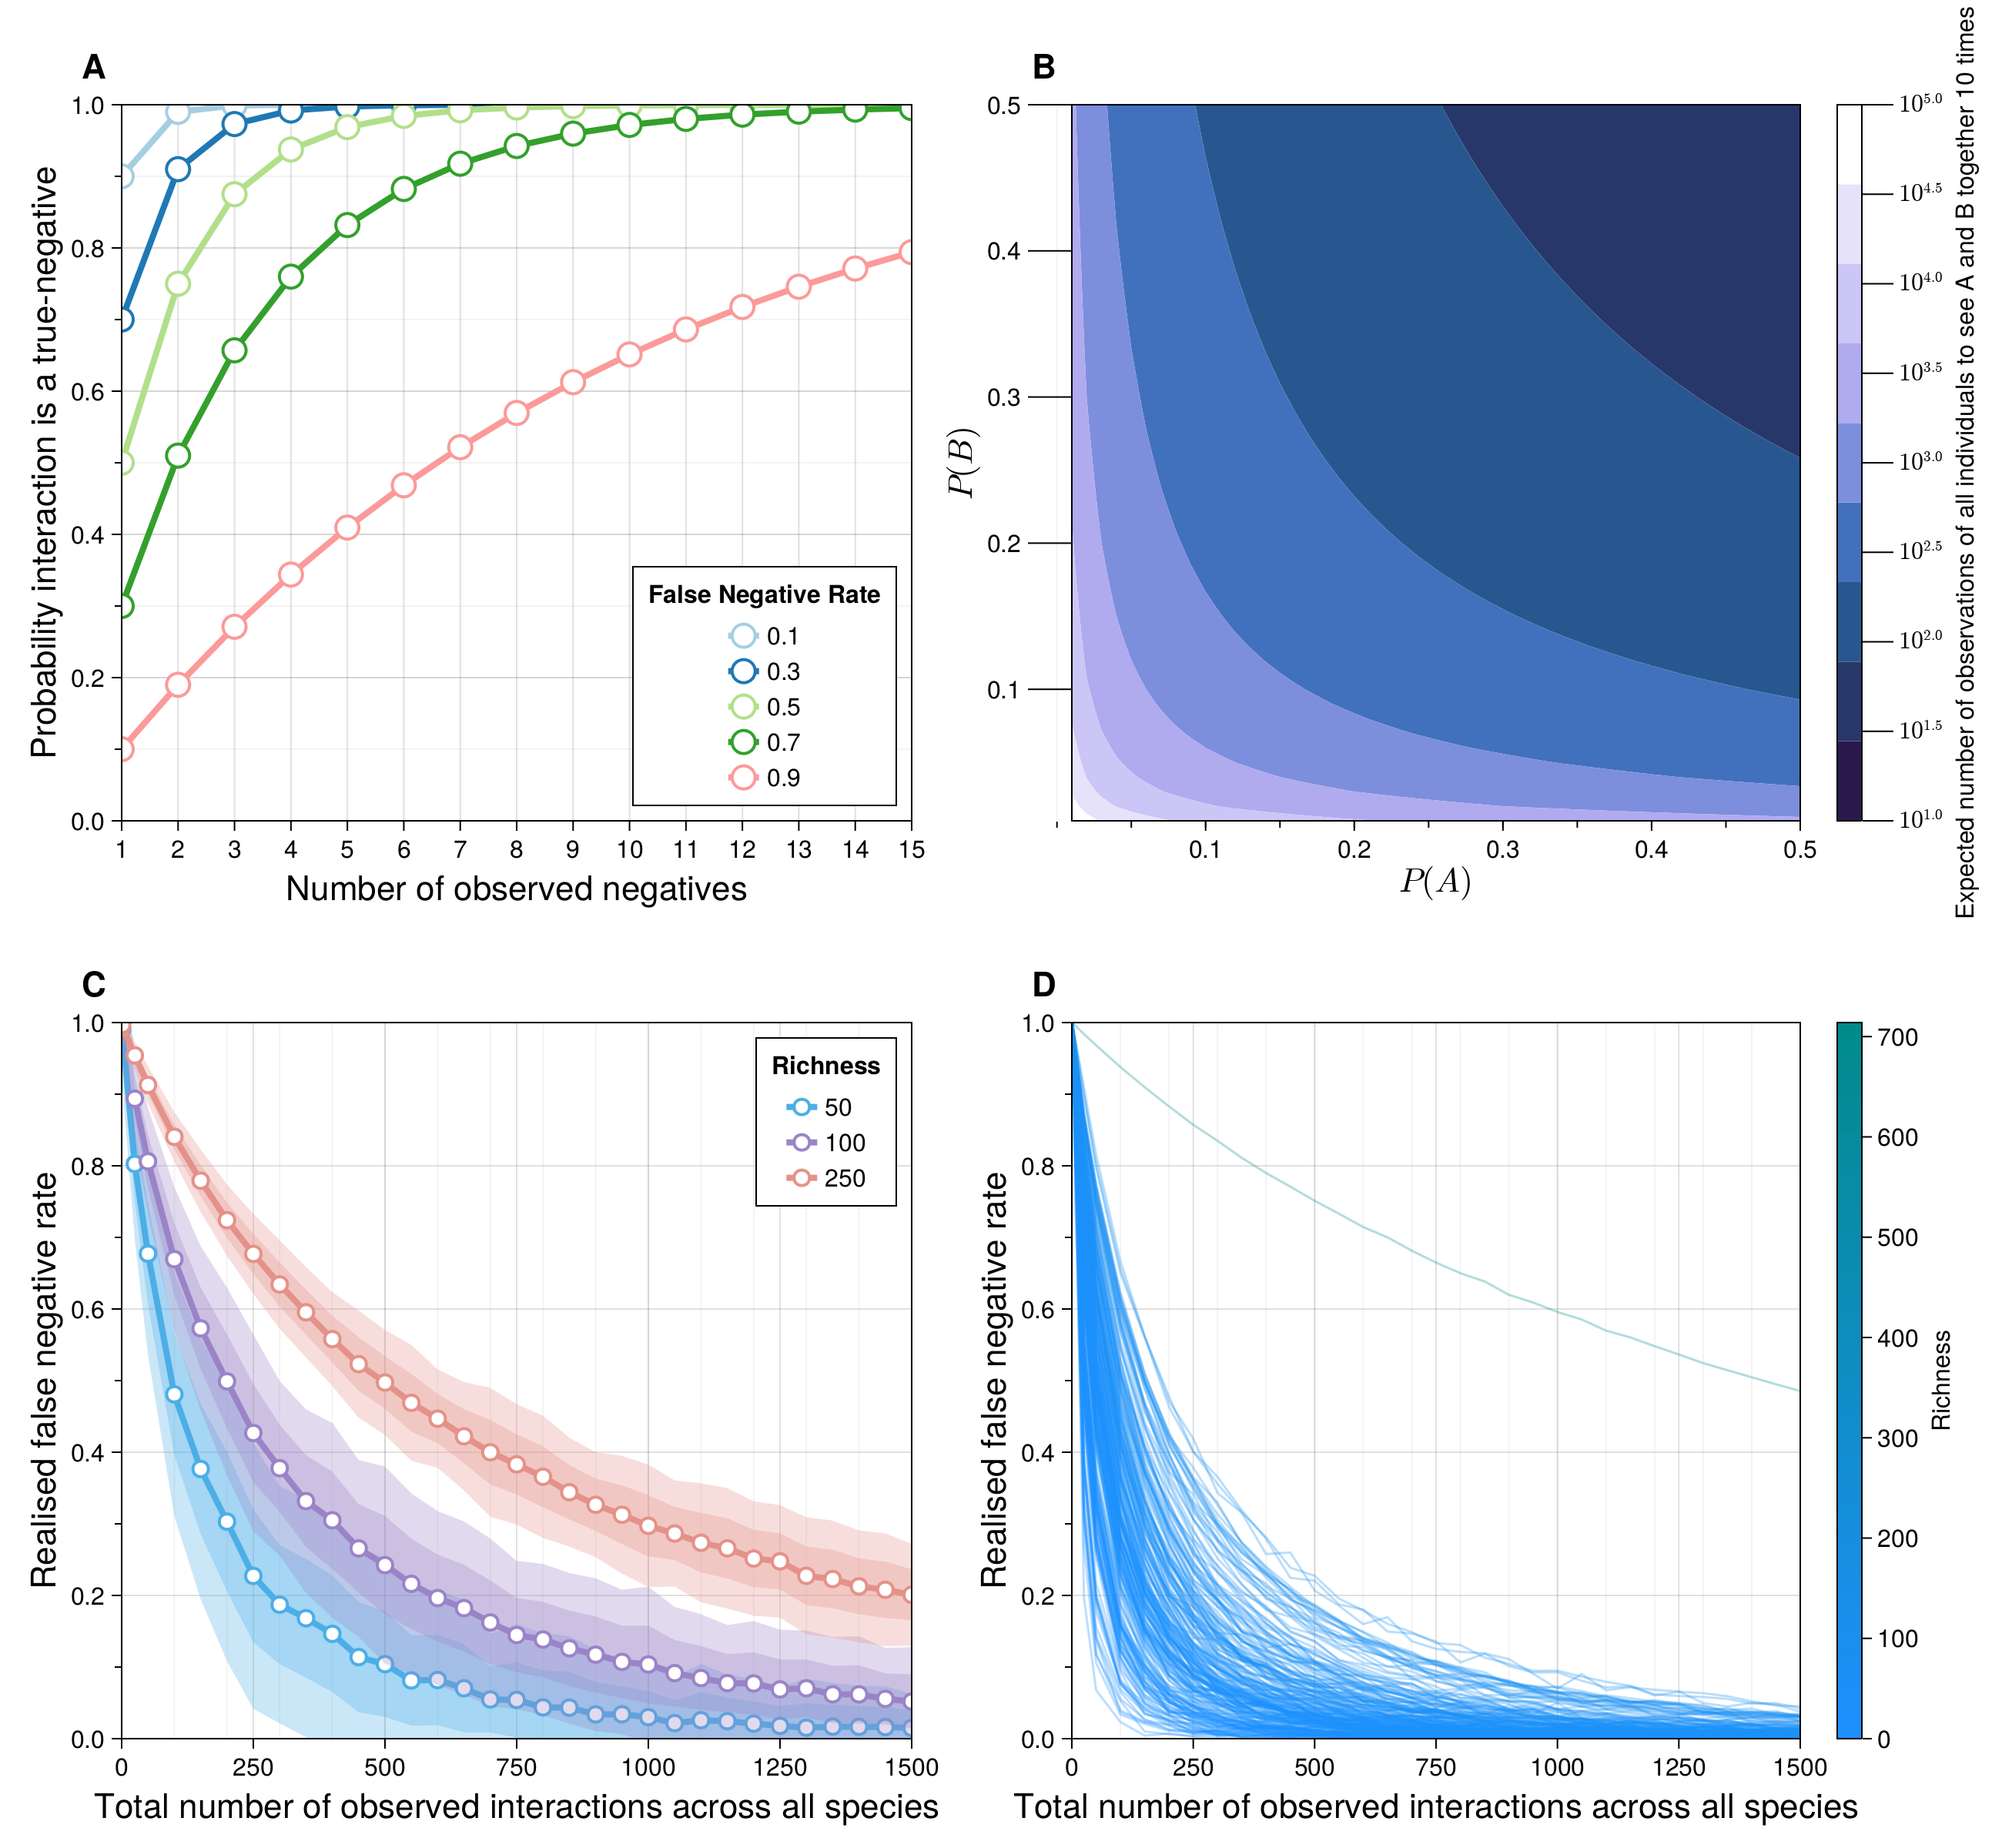
\includegraphics{./figures/fig1.png}
\caption{A) The probability an observed interaction is a true negative
(y-axis) given how many times it has been sampled as a non-interaction
(x-axis). Each color reflects a different value of \(p_{fn}\), the
false-negative rate (FNR). this is effectively the cdf of the
negative-binomial distribution with \(r=1\). (B) The expected needed
observations of all individuals of all species (y-axis) required to
obtain a goal number of observations (colors) of a particular species,
and a function of the relative abundance of that focal species (x-axis).
(C) and (D): False negative rate (y-axis) as a function of total
sampling effort (x-axis) and network size, computed using the method
described above. For 500 independent draws from the niche model
Williams2000SimRul at varying levels of species richness (colors) with
connectance drawn according to the flexible-links model
MacDonald2020RevLin as described in the main text. For each draw from
the niche model, 200 sets of 1500 observations are simulated, for which
each the mean false negative rate at each observation-step is computed.
Means denoted with points, with \(1\sigma\) in the first shade and
\(2\sigma\) in the second. B: empirical food webs from Mangal database
in teal, applied to the same process as the A. The outlier on panel B is
a 714 species food-web}\label{fig:fig1}
}
\end{figure}

In panel (c) of fig.~\ref{fig:totalobs}, we show the expected number of
total observations needed to obtain a ``goal'' number of observations
(colors) of a particular ``focal'' species. As an example, if we
hypothesize that \(A\) and \(B\) do not interact, and we want to see
species \(A\) and \(B\) both co-occurring and not-interacting 10 times
to be confident this is a negative (a la fig.~\ref{fig:negativebinom}),
then we need an expected 10,000 observations of all species if the
relative abundance of \(A\) is 0.00125.

Empirical data on interactions are subject to the practical limitations
of funding and human-work hours, and therefore existing data tend to
fall on the order on 100s or 1000s observations of individuals per site
(Nielsen \& Bascompte 2007; Schwarz \emph{et al.} 2020; Resasco \emph{et
al.} 2021). Clear aggregation of this data has proven difficult to find
and a meta-analysis of network data and sampling effort seems both
pertinent and necessary, in addition to the effects of aggregation of
interactions across taxonomic scales (Gauzens \emph{et al.} 2013;
Giacomuzzo \& Jordán 2021). Further, from fig.~\ref{fig:totalobs} it is
evident that the number of species considered in a study is inseparable
from the false-negative rate in that study, and this effect should be
taken into account when designing samples of ecological networks in the
future.

We conclude this section by advocating for the use of neutral models
similar to above to generate expectations about the number of
false-negatives in a data set of a given size. This could prove fruitful
both for designing surveys of interactions (Canard \emph{et al.} 2012),
but also because we may want to incorporate models of observation error
into predictive models (Joseph 2020). Additionally, one must consider
the context for sampling---is the goal to detect a particular species
\(A\) (as in fig.~\ref{fig:totalobs} (c)), or to get a representative
sample of interactions across the species pool? This argument is
well-considered when sampling species (Willott 2001), but has not yet
been internalized for designing samples of communities.

\hypertarget{positive-associations-can-increase-the-probability-of-false-negatives}{%
\subsection{Positive associations can increase the probability of
false-negatives}\label{positive-associations-can-increase-the-probability-of-false-negatives}}

This model above doesn't consider the possibility that there are
positive or negative associations which shift the probability of
observing two species together due to their interaction (Cazelles
\emph{et al.} 2016). However, here we demonstrate that the probability
of observing a false negative can be \emph{higher} if there is some
positive association between occurrence of species \(A\) and \(B\).

If we denote the probability that we observe an interaction we know
exists between \(A\) and \(B\) as \(P(AB)\), and if there is \emph{no}
association between the marginal probabilities of observing \(A\) and
observing \(B\), denoted \(P(A)\) and \(P(B)\) respectively, then the
probability of observing the interaction \(P(AB) = P(A)P(B)\). In the
other case where there \emph{is} some positive strength of association
between observing both \(A\) and \(B\) because this interaction is
``important'' for each species, then the probability of observation both
\(A\) and \(B\), \(P(AB)\), is greater than \(P(A)P(B)\) as \(P(A)\) and
\(P(B)\) are not independent and instead are positively correlated,
\emph{i.e.} \(P(AB) > P(A)P(B)\). In this case, the probability of
observing a false negative in our naive model from
fig.~\ref{fig:negativebinom} is \(p_{fn} = 1 - P(AB)\) which due to the
above inequality implies \(p_{fn} \geq 1 - P(A)P(B)\) which indicates
increasingly greater probability of a false negative as
\(P(AB) \to P(AB) \gg P(A)P(B)\).

However this does not consider variation in species abundance in space
and time, (Poisot \emph{et al.} 2015). If positive or negative
associations between species structure variation in the distribution of
\(P(AB)\) across space/time, then the spatial/temporal biases induced by
data collection would further impact the realized false negative rate,
as the probability of false negative would not be constant for each pair
of species across sites. To test for this association empirical data, we
use two datasets: a set of host-parasite interactions sampled across 51
sites with 327 total taxa (Hadfield \emph{et al.} 2014) and a set of 18
New Zealand freshwater stream food webs with 566 total taxa (Thompson \&
Townsend 2000). We simply compute the empirical marginal distribution of
species occurrence, and compare the product of the marginals,
\(P(A)P(B)\), to the empirical joint distribution \(P(AB)\).

\begin{figure}
\hypertarget{fig:associations}{%
\centering
\includegraphics{./figures/positiveassociations.png}
\caption{Top: Hadfield, Bottom: NZ Stream Foodwebs. Effectively a
version of Cazelles \emph{et al.} (2016) figure 1 panel A. Both
distributions have \(\mu \neq 0\) with
\(p < 10^{-50}\)}\label{fig:associations}
}
\end{figure}

In fig.~\ref{fig:associations}, both host-parasite system (top) and
food-web (bottom) exhibit these positive associations. There is no
reason to expect the strength of this association to be the same in
different systems. At the moment, computing this metric for all of the
networks in the Mangal database proves challenging as most data sets use
different taxonmic identifiers, often at different resolutions. These
particular datasets (Thompson \& Townsend 2000; Hadfield \emph{et al.}
2014) were usable because they already have been sorted to have a fixed
taxonomic backbone (as part of EcologicalNetworks.jl (Banville \emph{et
al.} 2021)). Applying this in bulk to Mangal food-webs presents the
difficulty of resolving different taxon identifiers across spatial
samples of species with to different resolutions, which is why we can't
simply apply this to the whole Mangal database---this highlights a
general problem of resolving taxonomic indentifiers which use different
names and different resolutions in different ecological datasets, which
is a problem that needs to be addressed for computational approaches to
scale up to the world of big-ecological-data we hope to build, although
this is a task that may be aided via natural-language-processing
methods.

\hypertarget{the-impact-of-false-negatives-on-network-analysis-and-prediction}{%
\section{The impact of false-negatives on network analysis and
prediction}\label{the-impact-of-false-negatives-on-network-analysis-and-prediction}}

We now transition toward assessing the effects of false negatives in
data on the properties of the networks which we derive from this
interaction data, and their effect on models for predicting interactions
in the future.

\hypertarget{effects-of-false-negatives-on-network-properties}{%
\subsection{Effects of false-negatives on network
properties}\label{effects-of-false-negatives-on-network-properties}}

Here we simulate the process of observation with error to generate
synthetic data with a known proportion of false negatives, and compare
the computed network properties of the original ``true'' network to the
computed properties of the ``observed'' network with added
false-negatives. In fig.~\ref{fig:properties} we see the mean-squared
error of connectance, mean degree-centrality, and spectral radius,
computed across 2000, 2000, and 300 replicates respectively at each
value of the false negative rate \(p_{fn}\). All replicates use random
food-webs simulated using the niche model (Williams \& Martinez 2000)
with \(100\) species and connectance drawn from the flexible-links model
(MacDonald \emph{et al.} 2020) as before.

\begin{figure}
\hypertarget{fig:properties}{%
\centering
\includegraphics{./figures/props_specrad.png}
\caption{The mean-squared error (y-axis) of various network properties
(different colors) across various simulated false-negative rates
(x-axis). Means denoted with points, with \(1\sigma\) in the first shade
and \(2\sigma\) in the second.}\label{fig:properties}
}
\end{figure}

We consider three properties: connectance, mean-degree-centrality, and
spectral radius, indicative of local, meso, and global structure.
Connectance is effectively a node-level property, a proxy for the degree
distribution. Degree-centrality captures a different aspect of network
structure than connectance, more indicative of meso-level properties
that describe local `regions' of nodes interact. Spectral radius
(equivalent to the magnitude of the largest eigenvalue of \(A\)) is a
measure of global structure, and demonstrates the most variability in
response to false-negatives. For example, if a false-negative splits a
metaweb into two components, spectral-radius becomes the largest
eigenvalue of each of those two components. Also note that the form of
this error function varies little as species richness changes
(\emph{supplemental figure 2}). Practically, fig.~\ref{fig:properties}
shows us that different scales of measuring network structure vary in
their response to false negatives---connectance responds roughly
linearly to false negatives, whereas mean-degree-centrality decisively
does not. This implies that false-negatives adversely could effect
indirect interactions (Williams \emph{et al.} 2002).

\hypertarget{effects-of-false-negatives-on-ability-to-make-predictions}{%
\subsection{Effects of false negatives on ability to make
predictions}\label{effects-of-false-negatives-on-ability-to-make-predictions}}

Here, we assess the effect of false negatives in data on our ability to
make predictions about interactions. The prevalence of false-negatives
in data is the catalyst for interaction prediction in the first place,
and as a result methods have been proposed to counteract this bias
(Stock \emph{et al.} 2017; Poisot \emph{et al.} 2021b). However, it is
feasible this could induce too much noise for a interaction prediction
model to detect the signal of interaction chance from to the latent
properties of each species derived from the empirical network if the
number of false-negatives in a dataset becomes too overwhelming.

To test this, we use the same predictive model and dataset as in Strydom
\emph{et al.} (2021) to predict a metaweb from various empirical slices
of the species pool observed across space. This dataset from Hadfield
\emph{et al.} (2014) describes host-parasite interaction networks
sampled across 51 sites. We partition the data into 80-20 training-test
split, and then seed the training data with false negatives varying
rates, but crucially do nothing to the test data. We use the same model,
a neural-network with 3 feed-forward layers to predict outputs based on
features extracted from co-occurence (see Strydom \emph{et al.} (2021)
for more details). The single modification we make to the model is not
enforcing a number of positives in the training data as this constraint
is eventually impossible for increasing FNR. In fig.~\ref{fig:rocpr}, we
show receiving-operating-characteristic (ROC) and precision-recall (PR)
curves for the model with varying levels of synthetic false-negatives
added to the data.

\begin{figure}
\hypertarget{fig:rocpr}{%
\centering
\includegraphics{./figures/rocpr_falsenegatives.png}
\caption{Receiver-operating-characteristic (left) and precision-recall
(right) curves for the model on varying levels of false-negatives in the
data (colors). For each value of FNR, we run 30 random training/test
splits on 80/20 percent of the data. Replica of figure 1 in Strydom
\emph{et al.} (2021)}\label{fig:rocpr}
}
\end{figure}

Interestingly, the performance of the model from Strydom \emph{et al.}
(2021) changes little with many added false-negatives, which is good
evidence in favor neural-networks as a class of model for interaction
detection. Again, similar to our caveat in the previous section, this
dazta is \emph{already} likely to have many false-negatives, so the
effects of adding more as we do in this illustration might be mitigated
because there are already non-simulated false-negatives in the original
data which impact the models performance, even in the \(p_{fn} = 0\)
case.

We conclude be proposing that simulating the effects of false negatives
in this way can serve as an additional validation tool when aiming to
detect structural properties of networks using generative null models
(Connor \emph{et al.} 2017), or when evaluating the robustness of a
predictive model.

\hypertarget{discussion}{%
\section{Discussion}\label{discussion}}

Here, we have demonstrated that we expect false-negatives in species
interaction datasets purely due to the distribution of abundances within
a community. Positive associations between species occurrence (Cazelles
\emph{et al.} 2016) can increase the realized false-negative rate if the
sampling effort is limited, and we have presented evidence of this
non-random structure of co-occurrence in two sets of
spatially-replicated ecological network samples. We have also shown that
false-negatives can cause varying responses in our measurements of
network properties and further could impact our ability to reliably
predict interactions, which highlights the need for further research
into methods for correcting this bias in existing data (Stock \emph{et
al.} 2017). A brief caveat here is that we do not consider the rate of
false-positives---in large part false-positives can be explained by
misidentification of species, although this could be a relevant
consideration in some cases.

What does the future hold for this research? A better understanding of
how false-negatives impact our analyses and prediction of ecological
networks is a practical necessity. False-negatives could pose a problem
for many forms of inference in network ecology. For example, if we aim
to measure structural or dynamic stability of a network, or to infer
indirect interactions (Williams \emph{et al.} 2002), these estimates
could be prone to error if the observed network is not sampled
``enough''. What exactly ``enough'' means is then specific to the
application, and should be assessed via methods like those here when
designing samples. Further, predictions about network rewiring (Thompson
\& Gonzalez 2017) due to a changing climate could be error-prone without
accounting for interactions that have not been observed but that still
may become climatically infeasible.

This highlights the need for a quantitatively robust approach samples
design: for interactions (Jordano 2016b) and otherwise (Carlson \emph{et
al.} 2020). The primary takeaway is that when planning the sampling
effort across sites, it is necessary to take both the size of the
species pool into account. Further, simulating the process of
observation could be a powerful tool for planing study design which
takes relative abundance into account, and provide a null baseline for
detection of interaction strength. A model similar to that here can and
should be used to provide a neutral expectation of true-negative
probability given a number of observations of individuals at a given
place and time.

As we derive from fig.~\ref{fig:negativebinom}, we can never guarantee
there are no false-negatives in data. In recent years, there has been
interest toward explicitly accounting for false-negatives in models
(Stock \emph{et al.} 2017; Young \emph{et al.} 2021), and toward a
predictive approach toward interactions ---rather than expect that our
samples can fully capture all interactions, we know that some
interactions between species will not be observed due to finite sampling
capacity, and instead we must impute the true metaweb of interactions
given a set of samples (Strydom \emph{et al.} 2021). As a result, better
predictive approaches are needed for interaction networks (Strydom
\emph{et al.} 2021), and building models that explicitly account for
observation error is a necessary step forward for predictive ecological
models (Johnson \& Larremore 2021; Young \emph{et al.} 2021). Neural
networks, like the one used to predict interactions in the above
section, have been used to reflect hidden states which account for
detection error in occupancy modeling (Joseph 2020), and could be
integrated in the predictive models of the future.

A better conceptual framework for designing surveys and monitoring
networks, and incorporating sequential observations over time is clearly
needed (Carlson \emph{et al.} 2020), combined with a meta-analysis of
sampling effort and taxonomic resolution in existing data. Incorporating
a better understanding of sampling effects and bias on both the future
design of biodiversity monitoring systems, and the predictive models we
wish to apply to this data, is imperative in making actionable
predictions about the future of ecological interactions on our planet.

\hypertarget{references}{%
\section*{References}\label{references}}
\addcontentsline{toc}{section}{References}

\hypertarget{refs}{}
\begin{CSLReferences}{1}{0}
\leavevmode\vadjust pre{\hypertarget{ref-Banville2021ManJl}{}}%
Banville, F., Vissault, S. \& Poisot, T. (2021).
\href{https://doi.org/10.21105/joss.02721}{Mangal.jl and
EcologicalNetworks.jl: Two complementary packages for analyzing
ecological networks in Julia}. \emph{Journal of Open Source Software},
6, 2721.

\leavevmode\vadjust pre{\hypertarget{ref-Becker2021OptPre}{}}%
Becker, D.J., Albery, G.F., Sjodin, A.R., Poisot, T., Bergner, L.M.,
Dallas, T.A., \emph{et al.} (2021).
\href{https://doi.org/10.1101/2020.05.22.111344}{Optimizing predictive
models to prioritize viral discovery in zoonotic reservoirs}.
\emph{bioRxiv}, 2020.05.22.111344.

\leavevmode\vadjust pre{\hypertarget{ref-Bezanson2015JulFre}{}}%
Bezanson, J., Edelman, A., Karpinski, S. \& Shah, V.B. (2015).
\href{https://arxiv.org/abs/1411.1607}{Julia: A Fresh Approach to
Numerical Computing}. \emph{arXiv:1411.1607 {[}cs{]}}.

\leavevmode\vadjust pre{\hypertarget{ref-Blanchet2020CooNot}{}}%
Blanchet, F.G., Cazelles, K. \& Gravel, D. (2020).
\href{https://doi.org/10.1111/ele.13525}{Co-occurrence is not evidence
of ecological interactions}. \emph{Ecology Letters}, 23, 1050--1063.

\leavevmode\vadjust pre{\hypertarget{ref-Boakes2015InfSpe}{}}%
Boakes, E.H., Rout, T.M. \& Collen, B. (2015).
\href{https://doi.org/10.1111/2041-210X.12365}{Inferring species
extinction: The use of sighting records}. \emph{Methods in Ecology and
Evolution}, 6, 678--687.

\leavevmode\vadjust pre{\hypertarget{ref-Canard2012EmeStr}{}}%
Canard, E., Mouquet, N., Marescot, L., Gaston, K.J., Gravel, D. \&
Mouillot, D. (2012).
\href{https://doi.org/10.1371/journal.pone.0038295}{Emergence of
Structural Patterns in Neutral Trophic Networks}. \emph{PLOS ONE}, 7,
e38295.

\leavevmode\vadjust pre{\hypertarget{ref-Carlson2020WhaWou}{}}%
Carlson, C.J., Dallas, T.A., Alexander, L.W., Phelan, A.L. \& Phillips,
A.J. (2020). \href{https://doi.org/10.1098/rspb.2020.1841}{What would it
take to describe the global diversity of parasites?} \emph{Proceedings
of the Royal Society B: Biological Sciences}, 287, 20201841.

\leavevmode\vadjust pre{\hypertarget{ref-Cazelles2016TheSpe}{}}%
Cazelles, K., Araújo, M.B., Mouquet, N. \& Gravel, D. (2016).
\href{https://doi.org/10.1007/s12080-015-0281-9}{A theory for species
co-occurrence in interaction networks}. \emph{Theoretical Ecology}, 9,
39--48.

\leavevmode\vadjust pre{\hypertarget{ref-Connor2017UsiNul}{}}%
Connor, N., Barberán, A. \& Clauset, A. (2017).
\href{https://doi.org/10.1371/journal.pone.0176751}{Using null models to
infer microbial co-occurrence networks}. \emph{PLOS ONE}, 12, e0176751.

\leavevmode\vadjust pre{\hypertarget{ref-deAguiar2019RevBia}{}}%
de Aguiar, M.A.M., Newman, E.A., Pires, M.M., Yeakel, J.D., Boettiger,
C., Burkle, L.A., \emph{et al.} (2019).
\href{https://doi.org/10.7717/peerj.7566}{Revealing biases in the
sampling of ecological interaction networks}. \emph{PeerJ}, 7, e7566.

\leavevmode\vadjust pre{\hypertarget{ref-Gauzens2013FooAgg}{}}%
Gauzens, B., Legendre, S., Lazzaro, X. \& Lacroix, G. (2013). Food-web
aggregation, methodological and functional issues. \emph{Oikos}, 122,
1606--1615.

\leavevmode\vadjust pre{\hypertarget{ref-Giacomuzzo2021FooWeb}{}}%
Giacomuzzo, E. \& Jordán, F. (2021).
\emph{\href{https://doi.org/10.1101/2021.04.18.440319}{Food web
aggregation: Effects on key positions}} (Preprint). Ecology.

\leavevmode\vadjust pre{\hypertarget{ref-Griffiths1998SamEff}{}}%
Griffiths, D. (1998).
\href{https://doi.org/10.1046/j.1365-2656.1998.00244.x}{Sampling effort,
regression method, and the shape and slope of sizeabundance relations}.
\emph{Journal of Animal Ecology}, 67, 795--804.

\leavevmode\vadjust pre{\hypertarget{ref-Hadfield2014TalTwo}{}}%
Hadfield, J.D., Krasnov, B.R., Poulin, R. \& Nakagawa, S. (2014).
\href{https://doi.org/10.1086/674445}{A Tale of Two Phylogenies:
Comparative Analyses of Ecological Interactions}. \emph{The American
Naturalist}, 183, 174--187.

\leavevmode\vadjust pre{\hypertarget{ref-Johnson2021BayEst}{}}%
Johnson, E.K. \& Larremore, D.B. (2021).
\href{https://doi.org/10.1101/2021.07.06.451319}{Bayesian estimation of
population size and overlap from random subsamples}. \emph{bioRxiv},
2021.07.06.451319.

\leavevmode\vadjust pre{\hypertarget{ref-Jordano2016ChaEco}{}}%
Jordano, P. (2016a).
\href{https://doi.org/10.1371/journal.pbio.1002559}{Chasing Ecological
Interactions}. \emph{PLOS Biology}, 14, e1002559.

\leavevmode\vadjust pre{\hypertarget{ref-Jordano2016SamNet}{}}%
Jordano, P. (2016b).
\href{https://doi.org/10.1111/1365-2435.12763}{Sampling networks of
ecological interactions}. \emph{Functional Ecology}.

\leavevmode\vadjust pre{\hypertarget{ref-Joseph2020NeuHie}{}}%
Joseph, M.B. (2020). \href{https://doi.org/10.1111/ele.13462}{Neural
hierarchical models of ecological populations}. \emph{Ecology Letters},
23, 734--747.

\leavevmode\vadjust pre{\hypertarget{ref-Kenall2014OpeFut}{}}%
Kenall, A., Harold, S. \& Foote, C. (2014).
\href{https://doi.org/10.1186/1471-2148-14-66}{An open future for
ecological and evolutionary data?} \emph{BMC Evolutionary Biology}, 14,
66.

\leavevmode\vadjust pre{\hypertarget{ref-MacDonald2020RevLin}{}}%
MacDonald, A.A.M., Banville, F. \& Poisot, T. (2020).
\href{https://doi.org/10.1016/j.patter.2020.100079}{Revisiting the
Links-Species Scaling Relationship in Food Webs}. \emph{Patterns}, 1.

\leavevmode\vadjust pre{\hypertarget{ref-Makiola2020KeyQue}{}}%
Makiola, A., Compson, Z.G., Baird, D.J., Barnes, M.A., Boerlijst, S.P.,
Bouchez, A., \emph{et al.} (2020).
\href{https://doi.org/10.3389/fenvs.2019.00197}{Key Questions for
Next-Generation Biomonitoring}. \emph{Frontiers in Environmental
Science}, 7.

\leavevmode\vadjust pre{\hypertarget{ref-Martinez1999EffSam}{}}%
Martinez, N.D., Hawkins, B.A., Dawah, H.A. \& Feifarek, B.P. (1999).
\href{https://doi.org/10.1890/0012-9658(1999)080\%5B1044:EOSEOC\%5D2.0.CO;2}{Effects
of Sampling Effort on Characterization of Food-Web Structure}.
\emph{Ecology}, 80, 1044--1055.

\leavevmode\vadjust pre{\hypertarget{ref-Moore2016OptEco}{}}%
Moore, A.L. \& McCarthy, M.A. (2016).
\href{https://doi.org/10.1111/2041-210X.12564}{Optimizing ecological
survey effort over space and time}. \emph{Methods in Ecology and
Evolution}, 7, 891--899.

\leavevmode\vadjust pre{\hypertarget{ref-Nielsen2007EcoNet}{}}%
Nielsen, A. \& Bascompte, J. (2007).
\href{https://doi.org/10.1111/j.1365-2745.2007.01271.x}{Ecological
networks, nestedness and sampling effort}. \emph{Journal of Ecology},
95, 1134--1141.

\leavevmode\vadjust pre{\hypertarget{ref-Paine1988RoaMap}{}}%
Paine, R.T. (1988). \href{https://doi.org/10.2307/1941141}{Road Maps of
Interactions or Grist for Theoretical Development?} \emph{Ecology}, 69,
1648--1654.

\leavevmode\vadjust pre{\hypertarget{ref-Poisot2021GloKno}{}}%
Poisot, T., Bergeron, G., Cazelles, K., Dallas, T., Gravel, D.,
MacDonald, A., \emph{et al.} (2021a).
\href{https://doi.org/10.1111/jbi.14127}{Global knowledge gaps in
species interaction networks data}. \emph{Journal of Biogeography},
jbi.14127.

\leavevmode\vadjust pre{\hypertarget{ref-Poisot2021ImpMam}{}}%
Poisot, T., Ouellet, M.-A., Mollentze, N., Farrell, M.J., Becker, D.J.,
Albery, G.F., \emph{et al.} (2021b).
\href{https://arxiv.org/abs/2105.14973}{Imputing the mammalian virome
with linear filtering and singular value decomposition}.
\emph{arXiv:2105.14973 {[}q-bio{]}}.

\leavevmode\vadjust pre{\hypertarget{ref-Poisot2015SpeWhy}{}}%
Poisot, T., Stouffer, D.B. \& Gravel, D. (2015).
\href{https://doi.org/10.1111/oik.01719}{Beyond species: Why ecological
interaction networks vary through space and time}. \emph{Oikos}, 124,
243--251.

\leavevmode\vadjust pre{\hypertarget{ref-Resasco2021PlaPol}{}}%
Resasco, J., Chacoff, N.P. \& Vázquez, D.P. (2021).
\href{https://doi.org/10.1002/ecy.3359}{Plantpollinator interactions
between generalists persist over time and space}. \emph{Ecology}, 102,
e03359.

\leavevmode\vadjust pre{\hypertarget{ref-Savage2004EffBod}{}}%
Savage, V.M., Gillooly, J.F., Brown, J.H., West, G.B. \& Charnov, E.L.
(2004). \href{https://doi.org/10.1086/381872}{Effects of Body Size and
Temperature on Population Growth.} \emph{The American Naturalist}, 163,
429--441.

\leavevmode\vadjust pre{\hypertarget{ref-Schwarz2020TemSca}{}}%
Schwarz, B., Vázquez, D.P., CaraDonna, P.J., Knight, T.M., Benadi, G.,
Dormann, C.F., \emph{et al.} (2020).
\href{https://doi.org/10.1111/oik.07303}{Temporal scale-dependence of
plantpollinator networks}. \emph{Oikos}, 129, 1289--1302.

\leavevmode\vadjust pre{\hypertarget{ref-Stephenson2020TecAdv}{}}%
Stephenson, P. (2020).
\href{https://doi.org/10.1016/j.cosust.2020.08.005}{Technological
advances in biodiversity monitoring: Applicability, opportunities and
challenges}. \emph{Current Opinion in Environmental Sustainability}, 45,
36--41.

\leavevmode\vadjust pre{\hypertarget{ref-Stock2017LinFil}{}}%
Stock, M., Poisot, T., Waegeman, W. \& De Baets, B. (2017).
\href{https://doi.org/10.1038/srep45908}{Linear filtering reveals false
negatives in species interaction data}. \emph{Scientific Reports}, 7,
45908.

\leavevmode\vadjust pre{\hypertarget{ref-Strydom2021RoaPre}{}}%
Strydom, T., Catchen, M.D., Banville, F., Caron, D., Dansereau, G.,
Desjardins-Proulx, P., \emph{et al.} (2021).
\emph{\href{https://doi.org/10.32942/osf.io/eu7k3}{A Roadmap Toward
Predicting Species Interaction Networks (Across Space and Time)}}
(Preprint). EcoEvoRxiv.

\leavevmode\vadjust pre{\hypertarget{ref-Thompson2017DisGov}{}}%
Thompson, P.L. \& Gonzalez, A. (2017).
\href{https://doi.org/10.1038/s41559-017-0162}{Dispersal governs the
reorganization of ecological networks under environmental change}.
\emph{Nature Ecology \& Evolution}, 1, 1--8.

\leavevmode\vadjust pre{\hypertarget{ref-Thompson2000ResSol}{}}%
Thompson, R.M. \& Townsend, C.R. (2000).
\href{https://doi.org/10.1046/j.1365-2427.2000.00579.x}{Is resolution
the solution?: The effect of taxonomic resolution on the calculated
properties of three stream food webs}. \emph{Freshwater Biology}, 44,
413--422.

\leavevmode\vadjust pre{\hypertarget{ref-Volkov2003NeuThe}{}}%
Volkov, I., Banavar, J.R., Hubbell, S.P. \& Maritan, A. (2003).
\href{https://doi.org/10.1038/nature01883}{Neutral theory and relative
species abundance in ecology}. \emph{Nature}, 424, 1035--1037.

\leavevmode\vadjust pre{\hypertarget{ref-Walther1995SamEff}{}}%
Walther, B.A., Cotgreave, P., Price, R.D., Gregory, R.D. \& Clayton,
D.H. (1995).
\href{https://doi.org/10.1016/0169-4758(95)80047-6}{Sampling Effort and
Parasite Species Richness}. \emph{Parasitology Today}, 11, 306--310.

\leavevmode\vadjust pre{\hypertarget{ref-Williams2002TwoDeg}{}}%
Williams, R.J., Berlow, E.L., Dunne, J.A., Barabasi, A.-L. \& Martinez,
N.D. (2002). \href{https://doi.org/10.1073/pnas.192448799}{Two degrees
of separation in complex food webs}. \emph{Proceedings of the National
Academy of Sciences}, 99, 12913--12916.

\leavevmode\vadjust pre{\hypertarget{ref-Williams2000SimRul}{}}%
Williams, R.J. \& Martinez, N.D. (2000).
\href{https://doi.org/10.1038/35004572}{Simple rules yield complex food
webs}. \emph{Nature}, 404, 180--183.

\leavevmode\vadjust pre{\hypertarget{ref-Willott2001SpeAcc}{}}%
Willott, S.J. (2001).
\href{https://doi.org/10.1046/j.1365-2664.2001.00589.x}{Species
accumulation curves and the measure of sampling effort}. \emph{Journal
of Applied Ecology}, 38, 484--486.

\leavevmode\vadjust pre{\hypertarget{ref-Young2021RecPla}{}}%
Young, J.-G., Valdovinos, F.S. \& Newman, M.E.J. (2021).
\href{https://doi.org/10.1038/s41467-021-24149-x}{Reconstruction of
plantpollinator networks from observational data}. \emph{Nature
Communications}, 12, 3911.

\end{CSLReferences}

\end{document}
